%
%
\documentclass{article}
\usepackage{amsmath}
\usepackage{graphicx}
\usepackage{color}
\usepackage{amsfonts}
\usepackage[margin=4cm]{geometry}
\newcommand{\cE}{\mathcal{E}}                               %
\newcommand{\cM}{\mathcal{M}}                               %
\newcommand{\cC}{\mathcal{C}}                               %
\newcommand{\cK}{\mathcal{K}}                               %
\newcommand{\bs}{\boldsymbol}                               %

\begin{document}

\title{Linear perturbation problem}
\author{Dominic Skinner}
\maketitle
Here we consider the linear perturbation problem, and how it can be solved
numerically. First we rescale into dimensionless parameters. Recall the full
equations are:
\begin{equation}
 \left( \begin{array}{c} p(z) \\ 0 \end{array} \right) =
\frac{E}{4\pi (1-\nu^2)} \int_0^{\infty} 
\underline{\underline{K}}(x-z) 
\left( \begin{array}{c} g'(x) \\ h'(x) \end{array} \right) dx
\end{equation}
\\
\begin{equation}
12\mu c = h^2 p'
\end{equation}
\\
\begin{equation}
\left\{ \begin{array}{ccc}
\displaystyle \lim_{x\to\infty} h''(x) & = & \frac{12(1-\nu^2)}{E\ell^3} M \\
\displaystyle \lim_{x\to\infty} g'(x) & = & \frac{6(1-\nu^2)}{E\ell^3} M 
\end{array} \right.
\end{equation}
\\
\begin{equation}
K_I = \lim_{x\to 0} \frac{E}{1-\nu^2} \sqrt{\frac{\pi}{8}} \sqrt{x} h'(x)
\end{equation}
\\
\section{Rescaling}
Let us use a length scale $\ell$, pressure scale $p^* = \frac{E}{12(1-\nu^2)}$,
and a time scale $t^* = 12\mu/p*$. We define the following dimensionless
parameters.
\[\cM = \frac{M}{p^* \ell^2}, \qquad \cC = \frac{c}{\ell/t^*} = \frac{12\mu c}
{p^* \ell}, \qquad \cK = \frac{K_I}{p^* \ell ^{1/2}} \]
We also define the variables (with $\alpha$ and $\beta$ dimensionless 
rescalings to be determined)
\[ x = \ell \xi, \qquad K_{ij} = \Lambda_{ij}/ \ell, \qquad
h = \alpha \ell H(\xi), \qquad p = \beta p^* \Pi ( \xi) \] 
So that
\[ \left( \begin{array}{c} \Pi \\ 0 \end{array} \right)
= \frac{3\alpha}{\pi\beta} \int \Lambda 
 \left( \begin{array}{c} G' \\ H' \end{array} \right) d\xi, \qquad
H^2 \Pi' = \frac{\cC}{\alpha^2 \beta}, \] \\
\[ H'' \to \cM/\alpha, \qquad
3\sqrt{2\pi\xi}H' \sim \frac{K_I}{(4\pi \mu x p^{*2} \ell^{1/2})^{1/3}} \]
\\
Choosing $\alpha = \pi \beta/3 = \cM$, $\displaystyle \lambda = 
\frac{\pi \cC}{3 \cM^3} = \frac{4\pi \mu c p^{*2} \ell^5}{M^3}$ gets 
Tim's scalings. 
\[ \left( \begin{array}{c} \Pi \\ 0 \end{array} \right)
= \int \Lambda 
 \left( \begin{array}{c} G' \\ H' \end{array} \right) d\xi, \qquad
H^2 \Pi' = \lambda, \] 
\[ H'' \to 1, \qquad
3\sqrt{2\pi\xi}H' \sim \frac{K_I}{M \ell^{-3/2}} \equiv \kappa \]
\\
Now suppose that $(G_0, H_0, \Pi_0, \lambda_0)$ gives the solution for 
$\kappa=0$. The outer limit of the LEFM solution is
\[ H \sim H_0 + \cE(\kappa) \left( \frac{\tilde{A} \lambda_1}{3\lambda_0^{2/3}}
\xi^{2/3} + \xi^s + \dots \right) \]
where $\cE = C \kappa^{4-6s} \lambda_0^{2s-1}$, $s = 0.138673$, and 
$C = \beta_1 (2/9\pi)^{2-3s}(1/4\pi)^{2-3s} = 8.99 \times 10^{-5}$.
Working to first order in $\cE$ we have the linear outer problem
\[ \left( \begin{array}{c} \Pi_1 \\ 0 \end{array} \right)
= \int \Lambda 
 \left( \begin{array}{c} G_1' \\ H_1' \end{array} \right) d\xi, \qquad
H_0^2 \Pi_1' + 2 H_0H_1 \Pi_0'= \lambda_1, \] 
\[ H_1'' \to 0, \qquad H_1 \sim \xi^s + \frac{\tilde{A} \lambda_1}{3 
\lambda_0^{2/3}} \xi^{2/3} \]
But we also have to zeroth order
\[ \left( \begin{array}{c} \Pi_0 \\ 0 \end{array} \right)
= \int \Lambda 
 \left( \begin{array}{c} G_0' \\ H_0' \end{array} \right) d\xi, \qquad
H_0^2 \Pi_0' = \lambda_0, \] 
\[ H_0'' \to 1, \qquad H_0 \sim \tilde{A} \lambda_0^{1/3} \xi^{2/3} \]
Subtracting a scaled version of the first order solution from the zeroth
order solution, we get that
\[ \left( \begin{array}{c} \Pi_0 - a \Pi_1 \\ 0 \end{array} \right)
= \int \Lambda 
 \left( \begin{array}{c} G_0'- aG_1' \\ H_0'-aH_1' \end{array} \right) d\xi, 
\quad H_0^2 (\Pi_0-a\Pi_1)'+2H_0(H_0 - a H_1)\Pi_0' = 3\lambda_0 - 
a \lambda_1, \] 
\[ (H_0-aH_1)'' \to 1, \qquad H_0 - a H_1 \sim 
\frac{\tilde{A}}{3 \lambda_0^{2/3}} \xi^{2/3}(3\lambda_0 - a\lambda_1) 
- a \xi^s\]
Setting $a = 3\lambda_0/\lambda_1$ and defining $\tilde{H} = 
H_0 - a H_1$ etc. gets the equations 
\[ \left( \begin{array}{c} \tilde{\Pi} \\ 0 \end{array} \right)
= \int \Lambda 
 \left( \begin{array}{c} \tilde{G}' \\ \tilde{H}' \end{array} \right) d\xi, 
\quad H_0^2 \tilde{\Pi}'+2H_0\tilde{H}\Pi_0' = 0, \] 
\[ \tilde{H}'' \to 1, \qquad \tilde{H} \sim - \frac{3\lambda_0}{\lambda_1} 
\xi^s \]
Note that this is a slightly different scaling than proposed before, but 
this has the same boundary conditions at $\infty$ as before, and
the elasticity integral equation is exactly the same as before. This means
the old code can hopefully be reused, as well as the fact that we can easily
impose conditions at $\infty$, whereas it is non-obvious how to easily impose 
them at 0.
\section{Numerical strategy}
The old method of linearising via $\tilde{H}'(\xi) \approx 
\frac{1}{\sqrt{\xi}}(a\xi+b)$ may no longer be too helpful, since we do not 
predict such a $\xi^{-1/2}$ singularity. It is possible (and even likely) 
that $\tilde{G}'$ still has such a singularity, but we predict $\tilde{H}'$ 
to have a $\xi^{s-1}$ singularity near the origin. The 
$\tilde{H}'(\xi) \approx \xi^{s-1}(a\xi+b)$ 
approximation, makes the analytic expressions inside the elasticity integal 
become worse than they already were.
\\
\\
For now, we propose sticking to the old scheme. Even though it doesn't correctly
predict the behaviour near zero, the code should be written to see if this works
at all. If it doesn't, then at least we have a rough structure of the code
which shouldn't be too time consuming to change for a new representation.
\\
\\
Since we are using the same representation as before, we get that 
\[ \left( \begin{array}{c} \tilde{\Pi}(z_1) \\ \vdots \\ \tilde{\Pi}(z_{n-1}) 
\\[4pt] 0 \\ \vdots \\ 0 \end{array} \right) =
\left( \begin{array}{ccc} B_{1,1} & \cdots & B_{1 , 2n} \\
\vdots & \ddots & \vdots \\ B_{2(n-1),1} & \cdots & B_{2(n-1) , 2n} 
\end{array}
\right) \bs{\gamma} = BT\bs{\theta} \]
Where $B$ is in lieu of the Kernel integral, $T$ is the interpolation matrix,
and recall that 
\[ \bs{\gamma} = (a_1, \dots, a_n, b_1, \dots , b_n, c_1, \dots, c_n, d_1, \dots 
 d_n) \]
\[ \bs{\theta} = (a_1\xi_1+b_1, \dots, a_n\xi_n+b_n,\dots , c_1\xi_1+d_1, \dots,
 c_n \xi_n +  d_n) \]
Now, the difference from before is that the second equation for $\tilde{\Pi}$ 
is linear in $\tilde{H}$. 
\[ \tilde{\Pi} = \int_z^{\infty} \frac{2 \tilde{H} \Pi_0'}{H_0} d\xi \]
So (after a struggle) one might be able to alternatively represent 
$\tilde{\Pi}$ via 
\[ \left( \begin{array}{c} \tilde{\Pi}(z_1) \\ \vdots \\ \tilde{\Pi}(z_{n-1}) 
\\[4pt] 0 \\ \vdots \\ 0 \end{array} \right) =
\left( \begin{array}{ccc} R_{1,1} & \cdots & R_{1 , 2n} \\
\vdots & \ddots & \vdots \\ R_{n-1,1} & \cdots & R_{n-1 , 2n} 
\\ 0 & \cdots & 0  \\
\vdots & \ddots & \vdots \\ 0 & \cdots & 0 
\end{array} \right) \bs{\theta} \]
To get that $(BT-R)\bs{\theta} = 0$. We can add another two rows to the
matrix by demanding $\theta_n=1/2$ and 
$\displaystyle \frac{\theta_{2n}-\theta_{2n-1}}{x_{2n}- x_{2n-1}}=1$.
This gives us a matrix equation to solve: $A \bs{\theta} = \bs{c}$, where
$\bs{c}=0$ except $c_n=1/2$, $c_{2n}=1$. Inverting $A$ should get the 
required answer, no iteration needed.
\section{Numerical Details}
We have inherited the matrix $BT$ from Tim's code. It may well be that this
needs changing in the future, but for now, we shall take this as given.
Therefore, the only real new part to code is the matrix $R$. 
\\
\\
Recall we have also inhereted a matrix $H_{Coeff}$. It has the property that
\[ ( w_1, e_1, r_1, \dots ,w_n, e_n, r_n ) = H_{Coeff} \bs{\theta} \]
We also recall that 
\[ \tilde{H}(\xi) = \left\{ \begin{array}{cc} \sqrt{\xi}(w_i\xi+e_i)+r_i &
i <t \\ w_i\xi^2+e_i\xi + r_i & i \geq t \end{array} \right. \]
For $\xi \in [\xi_i,\xi_{i+1}]$. We have that 
\[ (H(\xi_1), \dots, H(\xi_n) ) = S H_{coeff} \bs{\theta} \]
Where 
\[ S = \left( \begin{array}{*{14}{c}}
x_1^{3/2} & x_1^{1/2} & 1 & & & & & & & & & & 0 \\
 & & & \ddots \\
 & & & & x_{t-1}^{3/2} & x_{t-1}^{1/2} & 1 \\
 & & & & & & & x_{t}^{2} & x_{t} & 1 \\
 & & & & & & &  & & & \ddots \\
0 & & & & & & &  & & & &    x_{n}^{2} & x_{n} & 1 \\
\end{array} \right) \]
(This will never appear as a matrix in the code, point is that it can be
thought of one). Recall the equation we are trying to solve:
\[ \tilde{\Pi} = \int_z^{\infty} \frac{2 \tilde{H} \Pi_0'}{H_0} d\xi \]
We want to solve for $(\tilde{\Pi}(z_1), \dots \tilde{\Pi}(z_{n-1}))$.
In a break with the approaches previously used, we will solve this with
simple numerical integration via the trapezium rule. We will also use
the lubrication equation $\Pi_0'H_0^2=\lambda_0$ to remove $\Pi_0'$.
\[ \tilde{\Pi}(z_k) = \int_{z_k}^{\xi_{k+1}} \frac{2\lambda_0 \tilde{H}}{H_0^3} 
d\xi + \sum_{r=k+1}^{n-1}\int_{\xi_r}^{\xi_{r+1}} \frac{2\lambda_0 \tilde{H}}
{H_0^3} d\xi + \int_{\xi_n}^{\infty} \frac{2\lambda_0 \tilde{H}}
{H_0^3} d\xi\]
It is simple to approximate some of these integrals with the trapezium rule:
\[ \int_{\xi_r}^{\xi_{r+1}} \frac{2\lambda_0 \tilde{H}}{H_0^3} d\xi 
\approx (\xi_{r+1} - \xi_r)\left( \frac{\lambda_0\tilde{H}(\xi_{r+1})}
{H_0^3(\xi_{r+1})} + \frac{\lambda_0\tilde{H}(\xi_{r})}
{H_0^3(\xi_{r})} \right) =(\xi_{r+1} - \xi_r)(f(\xi_{r+1})+f(\xi_r)) \]
Where we adopt the new notation $f(\xi) = \lambda_0 \tilde{H}(\xi)/H_0^3(\xi)$
for convenience. It is easy to see that 
\[ (f(\xi_1), \dots , f(\xi_n)) = FSH_{Coeff}\bs{\theta} \] 
where now 
\[ F = \left( \begin{array}{ccc}
\lambda_0/H_0^3(\xi_1) \\
& \ddots \\
& & \lambda_0/H_0^3(\xi_n) \end{array} \right) \]
That leaves two integrals to deal with. The first is also easily despached
with the trapezium rule, just needs a little bit of care.
\[ \int_{z_k}^{\xi_{k+1}} 2f(\xi) d\xi \approx (\xi_{k+1} - z_k)(f(\xi_{k+1})
+ f(z_k) )\]
where
\[f(z_k) \approx f(\xi_k) + \frac{z_k - \xi_k}{\xi_{k+1}-\xi_k} (f(\xi_{k+1})
-f(\xi_k) ) \] 
so
\[ \int_{z_k}^{\xi_{k+1}} 2f(\xi) d\xi \approx (\xi_{k+1} - z_k)
\left( f(\xi_k) \frac{\xi_{k+1}-z_k}{\xi_{k+1}-\xi_k} + f(\xi_{k+1})
\frac{z_k - 2 \xi_k +\xi_{k+1}}{\xi_{k+1}-\xi_k} \right)
\]
\begin{figure}[!ht]\centering
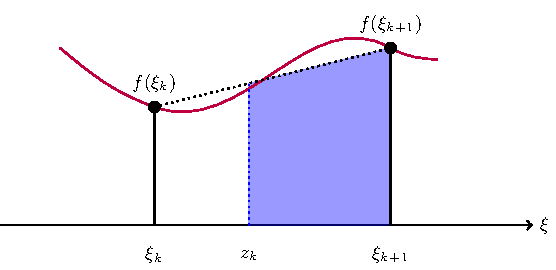
\includegraphics{LinFig1.pdf}
\end{figure}
\\
As for $ \int_{\xi_n}^{\infty} 2f(\xi) d\xi$, this is where I don't have any
particularly good ideas so far. From the boundary conditions, expect that
$f(\xi) \approx 4\lambda_0 /\xi^4$ to leading order. So
\[ \int_{\xi_n}^{\infty} 2f(\xi) d\xi \approx \frac{8\lambda_0}{4\xi_n^3}
= \frac{2}{3} \xi_n f(\xi_n)\]
This may prove to be a pretty poor approximation, so if this method fails, 
correcting this (or putting solid bounds on the error) is an important 
improvement to make. Finally we get that
\begin{align*}
\tilde{\Pi}(z_k) \approx &(\xi_{k+1} - z_k)
\left( f(\xi_k) \frac{\xi_{k+1}-z_k}{\xi_{k+1}-\xi_k} + f(\xi_{k+1})
\frac{z_k - 2 \xi_k +\xi_{k+1}}{\xi_{k+1}-\xi_k} \right) \\
&+ \sum_{r = k+1}^{n-1} (\xi_{r+1} - \xi_{r})(f(\xi_{r+1})+f(\xi_r)) + 
\frac{2}{3}\xi_n f(\xi_n)
\end{align*}
Which, one notes, is linear in the $f(\xi_k)$. Thus 
\[ (\tilde{\Pi}(z_1), \dots , \tilde{\Pi}(z_{n-1})) = QFSH_{Coeff}\bs{\theta} \] 
Where
\begin{align*}
 Q(k,:) =& \left(\underbrace{0, \dots , 0}_{k-1 \mbox{ times}}, (\xi_{k+1}-z_k) 
\frac{\xi_{k+1}-z_k}{\xi_{k+1}-\xi_k},  (\xi_{k+1}-z_k) \frac{z_k - 2 \xi_k 
+\xi_{k+1}}{\xi_{k+1}-\xi_k} + (\xi_{k+2}-\xi_{k+1}), \right. \\[4pt]
& \qquad\qquad \left. \xi_{k+3}-\xi_{k+1}, \dots, \xi_{n}-\xi_{n-2}, 
\xi_{n}-\xi_{n-1} + \frac{2}{3}\xi_n  \right)
\end{align*}
%
%
% References/Bibliography /////////////////////////////////////////////////////
%
%\clearpage 
%\begin{thebibliography}{9}  
%
%\bibitem{Pedlosky}
%Pedlosky, J.,
%\emph{Geophysical Fluid Dynamics,}
%Springer-Verlag,
%1979.
%
%
%\end{thebibliography}
\end{document}

